\documentclass[xcolor={usenames,dvipsnames,svgnames}, compress]{beamer}

\usepackage{booktabs}
\usepackage{dcolumn}
% \usepackage{colortbl}
\usepackage{hyperref}
\usepackage{amsmath}


\usetheme{enziteto}

\setbeamertemplate{headline}{}

\begin{document}

\title{Simplifying, Regularizing and Strengthening Sum-Product Network Structure Learning}
\author{Antonio  Vergari, Nicola  {Di Mauro} and Floriana Esposito}
\institute{Lacam$@$DIB$@$Uniba}
\institute{Università degli Studi di Bari}
\department{Dipartimento di Informatica}
\laboratory{LACAM}
\group{Machine Learning}
\institutelogo{
\includegraphics[width=25pt]{figures/unibaba}}
\lablogo{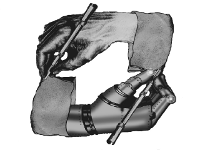
\includegraphics[width=35pt]{figures/lacam}}


{
  \setbeamertemplate{headline}{}
  \setbeamertemplate{footline}{}
  \begin{frame}
    \titlepage
  \end{frame}
}

\begin{frame}
  \frametitle{Tractable Probabilistic Graphical Models}
\end{frame}

\begin{frame}
  \frametitle{Sum-Product Networks (I)}
\end{frame}

\begin{frame}
  \frametitle{Sum-Product Networks (II)}
\end{frame}

\begin{frame}
  \frametitle{Structure Learning}
\end{frame}

\begin{frame}
  \frametitle{LearnSPN (I)}
\end{frame}

\begin{frame}
  \frametitle{LearnSPN (II)}
\end{frame}

\begin{frame}
  \frametitle{2 children}
\end{frame}

\begin{frame}
  \frametitle{Exp}
\end{frame}

\begin{frame}
  \frametitle{Early stopping}
\end{frame}

\begin{frame}
  \frametitle{Early stopping exp}
\end{frame}

\begin{frame}
  \frametitle{Bagging}
\end{frame}

\begin{frame}
  \frametitle{Bagging exp}
\end{frame}

\begin{frame}
  \frametitle{Conclusions and Further work}
\end{frame}

\end{document}

%%% Local Variables:
%%% mode: latex
%%% TeX-master: t
%%% TeX-engine: xetex
%%% End:
